
\documentclass[11pt, a4paper]{article}
\usepackage[T1]{fontenc}
\usepackage[utf8]{inputenc}
\usepackage[spanish]{babel}
\usepackage{mathpazo}
\usepackage{microtype}
\usepackage{amsmath, amssymb, bm}
\usepackage[margin=2.8cm]{geometry}
\usepackage{fancyhdr}
\usepackage{xcolor}
\usepackage{tcolorbox}
\usepackage{booktabs}
\usepackage{graphicx}
\usepackage{hyperref}
\usepackage{parskip}
\usepackage{caption}
\tcbuselibrary{most}

\definecolor{azulsuave}{RGB}{70,100,150}
\definecolor{azulclaro}{RGB}{230,238,250}
\definecolor{verdeclaro}{RGB}{230,248,236}
\definecolor{verdeoscuro}{RGB}{40,110,70}
\definecolor{amaclaro}{RGB}{255,250,225}
\definecolor{amaoscuro}{RGB}{160,120,20}
\definecolor{grisclaro}{RGB}{245,245,248}
\definecolor{grisoscuro}{RGB}{80,80,90}
\definecolor{rojoclaro}{RGB}{252,235,235}
\definecolor{rojooscuro}{RGB}{160,40,40}

\newtcolorbox{resultado}[1][]{
  colback=verdeclaro, colframe=verdeoscuro,
  fonttitle=\bfseries, title={#1}, boxrule=0.5pt,
  left=4pt, right=4pt, top=3pt, bottom=3pt}
\newtcolorbox{nota}[1][]{
  colback=amaclaro, colframe=amaoscuro,
  fonttitle=\bfseries, title={#1}, boxrule=0.5pt,
  left=4pt, right=4pt, top=3pt, bottom=3pt}
\newtcolorbox{cuidado}[1][]{
  colback=rojoclaro, colframe=rojooscuro,
  fonttitle=\bfseries, title={#1}, boxrule=0.5pt,
  left=4pt, right=4pt, top=3pt, bottom=3pt}

\hypersetup{colorlinks=true, linkcolor=azulsuave,
            urlcolor=azulsuave, citecolor=azulsuave}
\captionsetup{font=small, labelfont=bf}

\pagestyle{fancy}
\fancyhf{}
\fancyhead[L]{\small\color{grisoscuro}\textit{Proyecto KJM --- TES Colombia}}
\fancyhead[R]{\small\color{grisoscuro}\textit{Curva de Rendimientos DNS}}
\fancyfoot[C]{\thepage}
\renewcommand{\headrulewidth}{0.4pt}

\begin{document}

\begin{titlepage}
\centering
\vspace*{2cm}
{\LARGE\bfseries\color{azulsuave}
  Estimaci\'on de la Curva de Rendimientos\\[0.4em]
  de TES Colombia}\\[1.2em]
{\large Modelo: Dynamic Nelson-Siegel (DNS)}\\[0.5em]
{\large M\'etodo $\tau$: grid\_search}\\[2em]
\textcolor{azulsuave}{\rule{10cm}{0.8pt}}\\[1.5em]
{\large Kevin \& Juan David}\\[0.5em]
{\large Proyecto KJM --- Universidad}\\[0.5em]
{\large 16 de June de 2026}\\[2em]
\textcolor{grisoscuro}{\small
  Muestra: 2015-01-02 -- 2026-03-20\\
  Observaciones: 2735 d\'ias h\'abiles $\times$ 6 plazos
  (2, 3, 5, 7, 10, 15 a\~nos)
}
\end{titlepage}

\tableofcontents
\newpage

\section{Descripci\'on de los Datos}

La muestra cubre bonos TES colombianos en los plazos
2, 3, 5, 7, 10, 15 a\~nos, con observaciones diarias (d\'ias h\'abiles BVC)
desde 2015-01-02 hasta 2026-03-20, para un total de $T = 2735$ periodos
y $N = 6$ plazos.

\begin{nota}[Convenci\'on de unidades]
Los rendimientos est\'an expresados en porcentaje anual.
Los residuos y RMSE se reportan en puntos b\'asicos (pb = \% $\times$ 100).
\end{nota}

\begin{figure}[htbp]
\centering
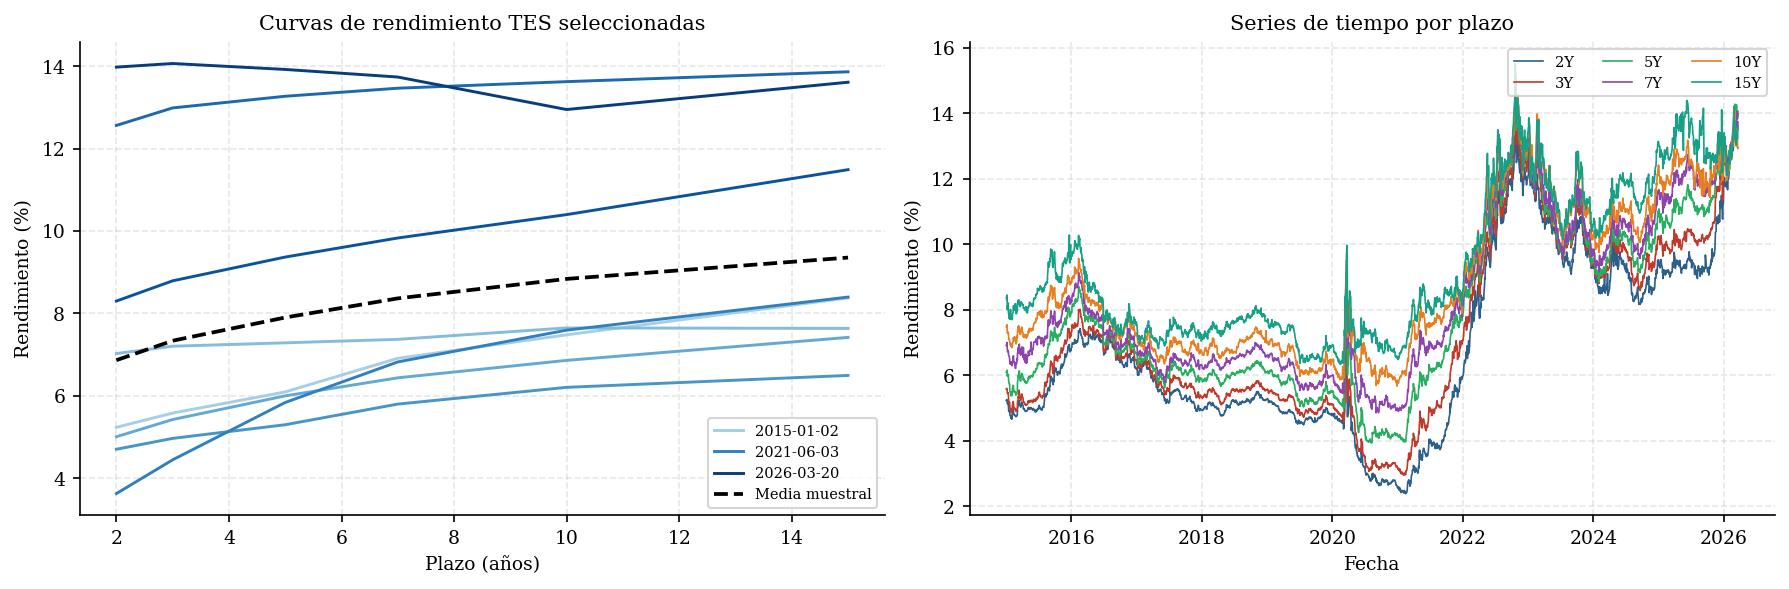
\includegraphics[width=\linewidth]{figures/fig_yield_curves.png}
\caption{Curvas de rendimiento TES seleccionadas (izquierda)
          y series de tiempo por plazo (derecha).}
\label{fig:yield_curves}
\end{figure}

\section{Especificaci\'on del Modelo}

\subsection{Ecuaci\'on de Medici\'on}

\begin{equation}
y_t(m) = \beta_{1t} + \beta_{2t}\left(\frac{1-e^{-m/\tau}}{m/\tau}\right)+ \beta_{3t}\left(\frac{1-e^{-m/\tau}}{m/\tau}- e^{-m/\tau}\right) + \varepsilon_t(m)
\end{equation}

donde $\boldsymbol{\beta}_t = (\beta_{1t}, \beta_{2t}, \beta_{3t})^\top$
son los factores latentes de nivel, pendiente y curvatura respectivamente,
y $\varepsilon_t(m) \sim \mathcal{N}(0, \sigma^2_m)$.

\subsection{Ecuaci\'on de Transici\'on}

\begin{equation}
\boldsymbol{\beta}_t - \boldsymbol{\mu} =
\mathbf{F}(\boldsymbol{\beta}_{t-1} - \boldsymbol{\mu}) + \boldsymbol{\eta}_t,
\qquad \boldsymbol{\eta}_t \sim \mathcal{N}(\mathbf{0}, \mathbf{Q})
\end{equation}

donde $\boldsymbol{\mu}$ es la media incondicional de los factores y
$\mathbf{F}$ es diagonal (Caldeira et al., 2010; \c{C}akmaklı, 2013).
\section{Resultados --- Kalman Filter (Frecuentista)}


    \subsection{Par\'ametros MLE}

    Log-verosimilitud marginal (KF): $\hat{\ell} = 10,282.25$.

    \begin{table}[htbp]
\centering
\small
\caption{Parametros MLE: media incondicional, persistencia y ruido de transicion.}
\label{tab:mle_params}
\begin{tabular}{lrrr}
\toprule
Factor & $\mu_i$ & $f_i$ & $\sqrt{q_i}$ (pb) \\
\midrule
$\beta_1$ & 10.6173 & 0.9950 & 9.5630 \\
$\beta_2$ & -4.3144 & 0.9950 & 12.6463 \\
$\beta_3$ & -1.3218 & 0.9950 & 29.4636 \\
\bottomrule
\end{tabular}
\end{table}

    \medskip
    \noindent Desviaciones est\'andar de medicion $\sqrt{R_{mm}}$ (pb):
    4.639, 12.151, 3.651, 11.692, 19.108, 11.302.

\subsection{Evoluci\'on de $\tau$}

\begin{figure}[htbp]
\centering
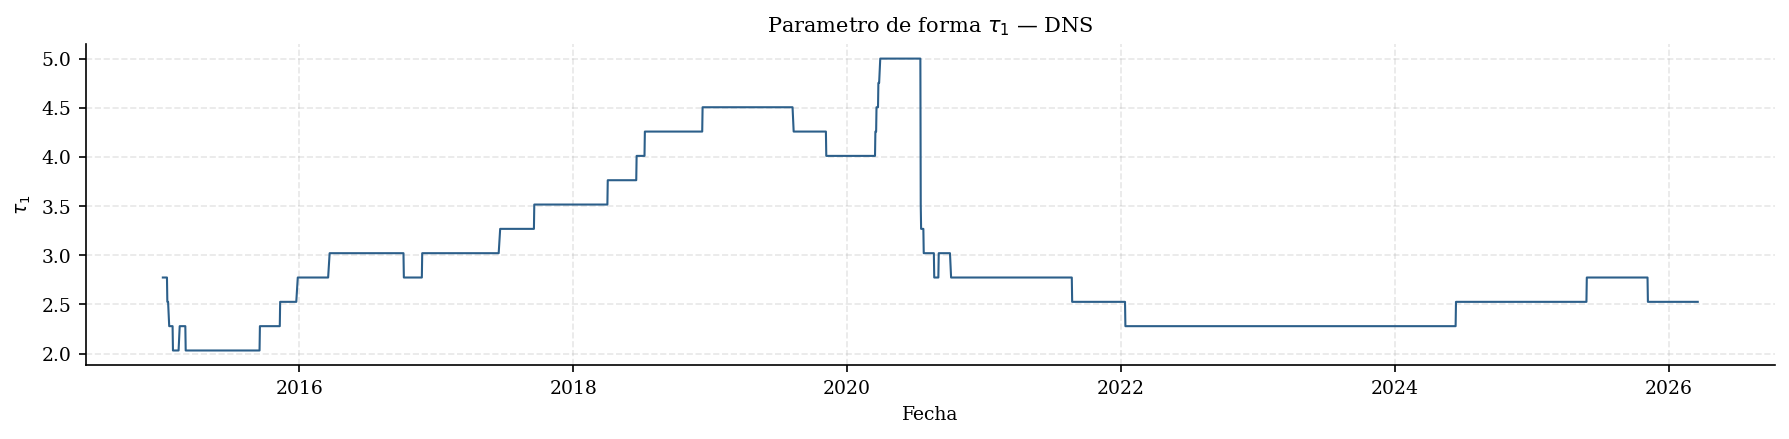
\includegraphics[width=\linewidth]{figures/fig_tau.png}
\caption{Evoluci\'on temporal del par\'ametro de forma $\tau$
          estimado via grid search adaptativo.}
\label{fig:tau}
\end{figure}

\subsection{Factores Latentes (Estados Suavizados)}

\begin{figure}[htbp]
\centering
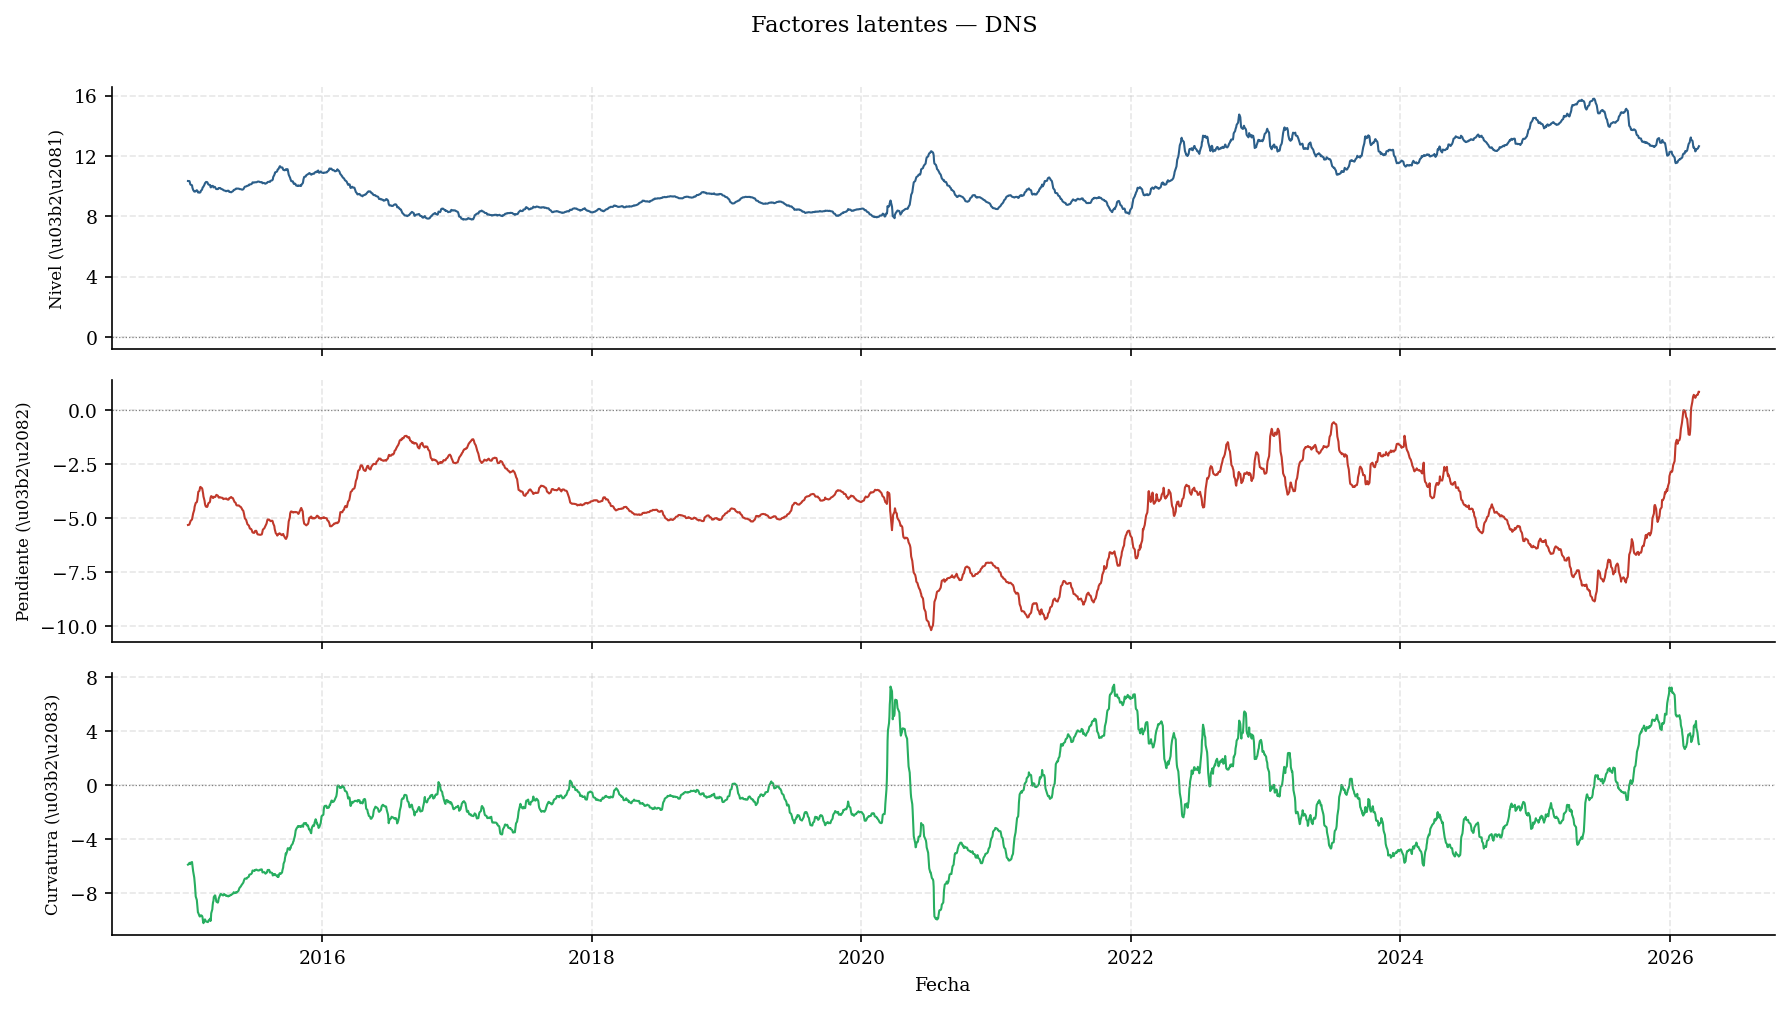
\includegraphics[width=\linewidth]{figures/fig_factors.png}
\caption{Factores latentes estimados via RTS Smoother.
          $\beta_1$: nivel, $\beta_2$: pendiente, $\beta_3$: curvatura.}
\label{fig:factors}
\end{figure}
\section{Diagn\'ostico de Residuos}

\begin{table}[htbp]
\centering
\small
\caption{Estadisticos de residuos de medicion por plazo (pb).}
\label{tab:residuals}
\begin{tabular}{lrrrrrrr}
\toprule
Plazo & RMSE & MAE & Sesgo & JB_pval & LB_pval & Normal & Blanco \\
\midrule
2Y & 3.2205 & 2.0075 & -0.4909 & 0.0000 & 0.0000 & No & No \\
3Y & 11.8344 & 8.7119 & 6.9100 & 0.0000 & 0.0000 & No & No \\
5Y & 2.3719 & 1.5932 & -0.3119 & 0.0000 & 0.0000 & No & No \\
7Y & 11.3102 & 8.6836 & -0.6868 & 0.0000 & 0.0000 & No & No \\
10Y & 18.7923 & 13.7246 & -2.1729 & 0.0000 & 0.0000 & No & No \\
15Y & 10.3333 & 6.7698 & 1.3271 & 0.0000 & 0.0000 & No & No \\
\bottomrule
\end{tabular}
\end{table}


\begin{figure}[htbp]
\centering
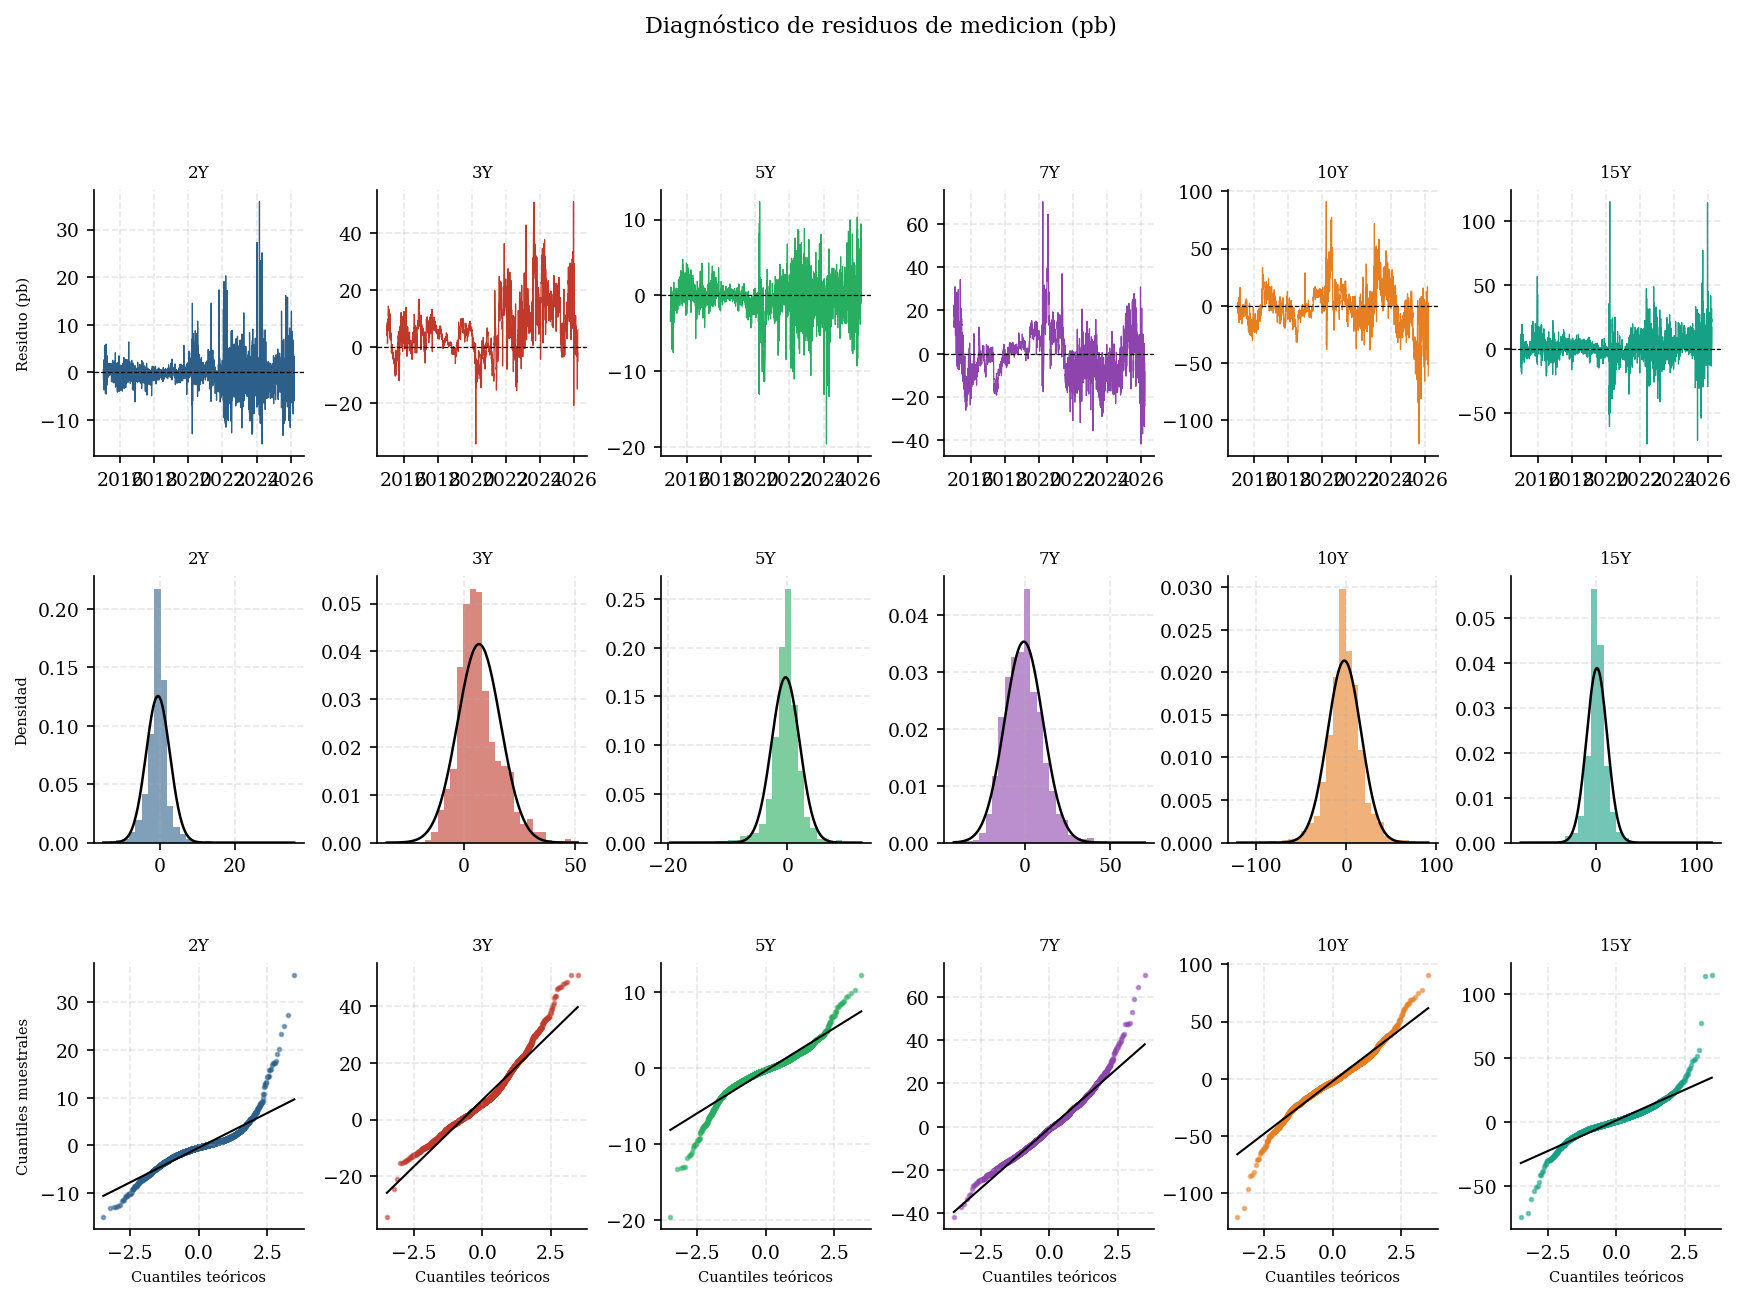
\includegraphics[width=\linewidth]{figures/fig_residuals.png}
\caption{Diagn\'ostico de residuos: series temporales (fila 1),
          histogramas con curva normal (fila 2), QQ-plots (fila 3).}
\label{fig:residuals}
\end{figure}

\section{Referencias}

\begin{itemize}
\item Nelson, C.\ \& Siegel, A.\ (1987). Parsimonious modeling of yield curves.
      \textit{Journal of Business}, 60(4), 473--489.
\item Svensson, L.\ (1994). Estimating and interpreting forward interest rates.
      \textit{NBER Working Paper}, 4871.
\item Diebold, F.\ \& Li, C.\ (2006). Forecasting the term structure of
      government bond yields.
      \textit{Journal of Econometrics}, 130(2), 337--364.
\item Caldeira, J., Laurini, M.\ \& Portugal, M.\ (2010).
      Bayesian inference applied to dynamic Nelson-Siegel model.
      \textit{Brazilian Review of Econometrics}.
\item \c{C}akmaklı, C.\ (2013). Bayesian semiparametric dynamic Nelson-Siegel model.
      \textit{Working Paper}.
\item Carter, C.\ \& Kohn, R.\ (1994). On Gibbs sampling for state space models.
      \textit{Biometrika}, 81(3), 541--553.
\item Hamilton, J.\ (1994). \textit{Time Series Analysis}. Princeton University Press.
\end{itemize}

\end{document}
